\section{Tipos de Modelo}\label{sec:tipos-de-modelo}
% TODO: adicionar figuras

É importante saber diferenciar os modelos devido ao método de resolução que varia para cada um deles.

\subsection{Modelo Linear × Não-linear}\label{subsec:modelo-linear}


Modelos lineares possuem como função objetivo uma função linear e todas as restrições também são lineares.
Exemplos:

\begin{itemize}
    \item $f(x) = ax + b$.
    \item $f(x_1, x_2) = x_1 + x_2 - 5$.
\end{itemize}

Já os não-lineares não obedecem essa regra, podendo ter suas variáveis se multiplicando ou funções trigonométricas e logarítmicas.
Exemplos:

\begin{itemize}
    \item $f(x_1, x_2) = x_1^2 + x_2^2$.
    \item $f(x_1, x_2) = \tan(x_1 + x_2)$.
\end{itemize}

\subsection{Modelo Contínuo × Discreto}\label{subsec:modelo-continuo-x-discreto}

Um modelo é contínuo quando sua região factível é contínua, ou seja, dado um ponto dessa região todos os seus vizinhos também serão uma solução.
Modelos discretos não possuem seu domínio contínuo.
A \autoref{fig:continuo-discreto} mostra um gráfico com exemplos de um modelo contínuo e outro discreto.

\begin{figure}[!htb]
    \centering
    \caption{Exemplo de modelo contínuo e discreto.}
    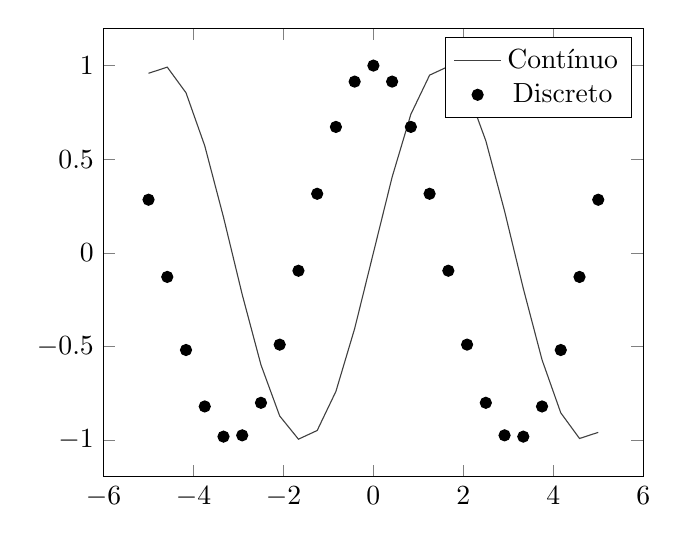
\begin{tikzpicture}
    \begin{axis}
        \addplot[darkgray] {sin((deg(x))};
        \addplot[black, only marks] {cos(deg(x))};
        \legend{Contínuo, Discreto}
    \end{axis}
\end{tikzpicture}

    \label{fig:continuo-discreto}
    \fonte{feito pelo autor.}
\end{figure}


\subsection{Modelo Determinístico × Estocástico}\label{subsec:modelo-deterministico-x-estocastico}

Em modelos determinísticos seus dados são conhecidos, enquanto os estocásticos possuem uma incerteza quanto aos dados.

\subsection{Tipos de Programação}\label{subsec:tipos-de-programacao}

Com base nas categorias de modelo é possível também dividir métodos de programação (planejamento) para sua solução.

\begin{itemize}
    \item Linear: modelo linear contínuo determinístico.
    \item Inteira: modelo linear discreto determinístico.
    \item Estocástica: modelo linear contínuo estocástico.
    \item Não-linear: modelo não-linear contínuo determinístico.
\end{itemize}
